\section{Descrição do Problema}

\subsection{Grafos e Redes Muiltimodais}
\frame
{
\frametitle{Grafos}
\begin{columns}[c]
\column{1.5in}
	\begin{align*}
		& G = (V,E) \\
		& V = \{1,2,3,4\} \\
		& E = \{e_1,e_2,e_3,e_4\}
	\end{align*}
\column{1.5in}
	\begin{figure}
		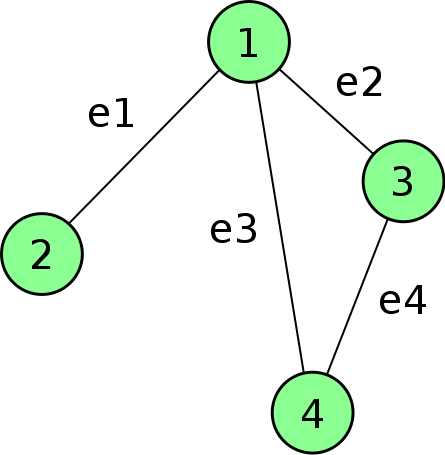
\includegraphics[width=\textwidth]{./imgs/grafo.png}
		\caption{Exemplo de grafo}
		%TODO: ref
		%\fonte{\citeonline{wikigrafo}}
	\end{figure}
\end{columns}
}

\frame
{
\frametitle{Redes Multimodais}
\begin{itemize}
	\item oi
\end{itemize}
}
